\begin{figure}
	\label{fig:histogram}
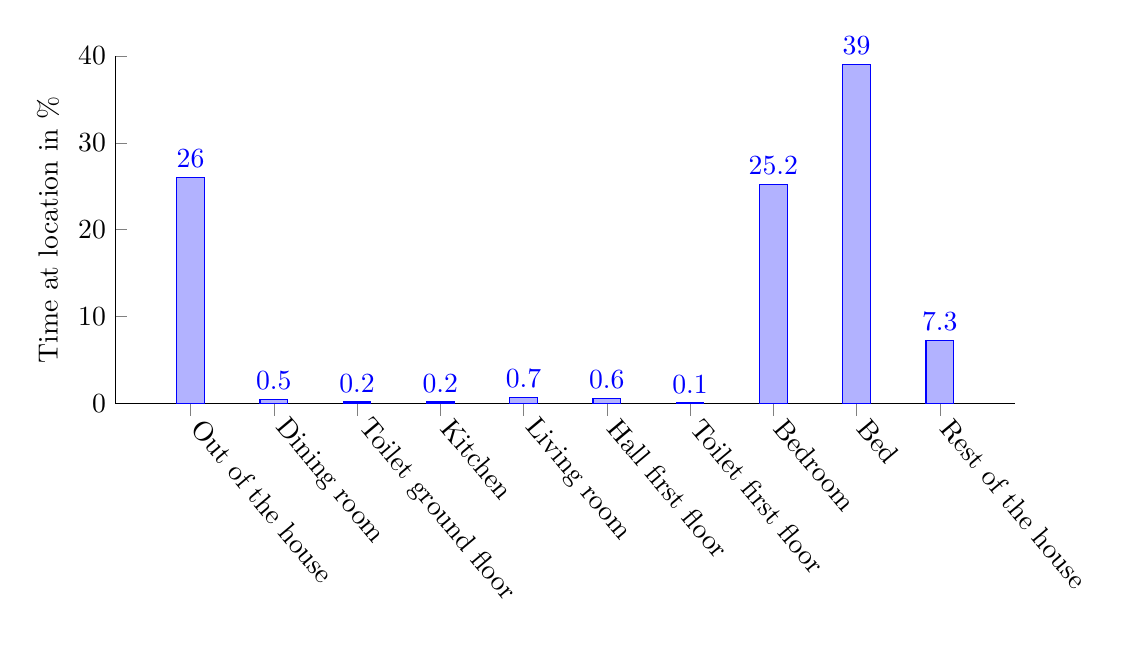
\begin{tikzpicture}
  \centering
  \begin{axis}[
        ybar,
    height=6cm,
    width=13cm,
    enlarge y limits=false,
    axis lines*=left,
    ymin=0,
    ymax=40,
     legend style={at={(0.5,-0.2)},
        anchor=north,legend columns=-1},
        ylabel={Time at location in \%},
        symbolic x coords={Out of the house, Dining room, Toilet ground floor, Kitchen, Living room, Hall first floor, Toilet first floor, Bedroom, Bed, Rest of the house},
     xtick=data,
	x tick label style = {rotate=-50, anchor = west},
        nodes near coords,
    every node near coord/.append style={
        anchor=south,
        rotate=0
    }
    ]
    \addplot coordinates {
	(Out of the house, 26) (Dining room, 0.5) (Toilet ground floor, 0.2) 
	(Kitchen, 0.2) (Living room, 0.7) (Hall first floor, 0.6)
	(Toilet first floor, 0.1) 
	(Bedroom, 25.2) (Bed, 39.0) (Rest of the house, 7.3)
	};
    
  \end{axis}
\end{tikzpicture}
	\caption{Histogram with the time been at the locations.}
\end{figure}
